\documentclass[9pt]{beamer}
\usepackage[utf8]{inputenc}
\usepackage{pslatex}
%% \usetheme[nat, greybg]{Frederiksberg}
\usetheme[nat]{Frederiksberg}
%% \usetheme[nat,wmark,logoplace=left,style=simple]{Frederiksberg}
%% \usetheme[nat,logoplace=left,style=simple]{Frederiksberg}

\usepackage{amsmath}
\usepackage{amssymb}
\usepackage{amsthm}
\usepackage{listings}
\usepackage{subcaption}
\usepackage{caption}
\usepackage{subcaption}

\graphicspath{ {imgs/} } 


\title{Breaks For Additive Season and Trend (BFAST)}
\subtitle{Theoretical background and results}
\institute{Department of Computer Science}
\author{Dmitry Serykh}
\date{\today}

\begin{document}

\frame[plain]{\titlepage}

\begin{frame}
\frametitle{Introduction}
\begin{itemize}
\item 7.5 ECTS project from Block 5
\item Two variants of the BFAST algorithm:
  \begin{itemize}
  \item The original BFAST (not to be confused with BFAST Monitor)
  \item BFAST0n: a lightweight version of BFAST
  \end{itemize}
\item Describe the underlying theory behind the main algorithm steps
\item Implement BFAST and BFAST0n in Python
\item Validate the implementation on multiple datasets, including datasets from
  the original paper by Verbesselt et al.
\item Foundation for a parallel BFAST implementation in the future
\end{itemize}
\end{frame}

\begin{frame}
  \frametitle{Ordinary Least Squares (OLS) Regression - Quick Recap}
  \begin{itemize}
    \item Linear Model
      \[
      \mathrm{Y} = \mathrm{X}\beta + \varepsilon
      \]
    \item Wish to find a solution to a quadratic minimization problem
      \[
      \hat{\beta} = \operatorname{argmin}_{\beta} \|Y-\mathrm{X} \boldsymbol{\beta}\|^{2}
      \]
    \item $\hat{\beta}$ is the OLS estimator for $\beta$ and can be found using the explicit formula:
      \[
      \hat{\boldsymbol{\beta}}=\left(\mathrm{X}^{\top} \mathrm{X}\right)^{-1}\mathrm{X}^{\top} \mathrm{Y}
      \]
    \item A numerically stable solution can be obtained using QR-decomposition or Moore-Penrose
      pseudoinverse of $\mathrm{X}$ (an expansive topic in itself).
  \end{itemize}
\end{frame}

\begin{frame}
\frametitle{OLS-Regression for Non-linear Functions}
\begin{itemize}
\item Linear regression can be used to estimate linear parameters for
  non-linear functions.
\item E.g. $f(x) = 25 + 2x^{1.2} + 3 \sin{x}$, then:
  \[
  \mathrm{X} = 
  \begin{bmatrix}
    1 & x_1^{1.2} & \sin{x_1}\\
    1 & x_2^{1.2} & \sin{x_2}\\
    \vdots & \vdots & \vdots \\
    1 & x_n^{1.2} & \sin{x_n}
  \end{bmatrix}
  \quad
  \beta =
  \begin{bmatrix}
    25 \\
    2 \\
    3
  \end{bmatrix}
  \]
\end{itemize}
\end{frame}


\begin{frame}
  \frametitle{OLS Example}
  \begin{figure}[H]
    \centering
    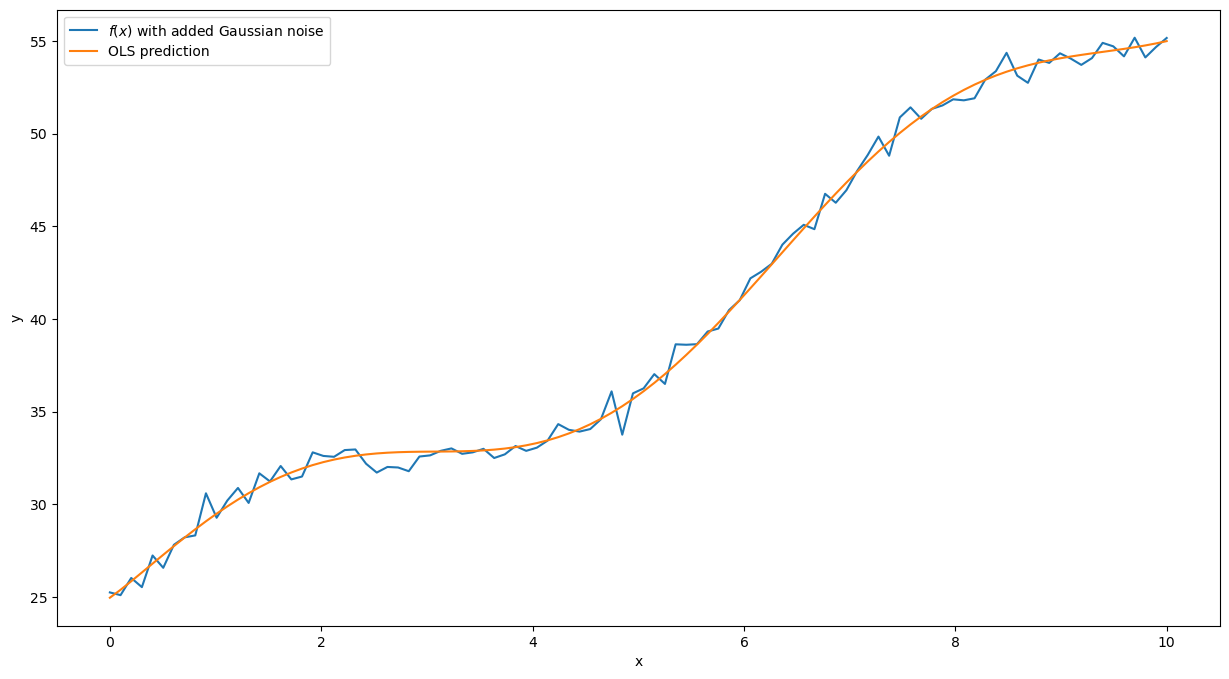
\includegraphics[width=0.8\textwidth]{imgs/ols1.png}
  \end{figure}
\end{frame}

\begin{frame}
\frametitle{STL Intro}
\begin{itemize}
\item Seasonal and Trend decomposition using Loess (STL), as first described by Cleveland et al.
\item Decomposition of a time series ($Y_v$) into a trend ($T_v$), seasonal ($S_v$) and remainder
  ($R_v$) s.t:
  \[
  Y_v = T_v + S_v + R_v \text{ for } v \in 1 \hdots N
  \]
\end{itemize}
\end{frame}

\begin{frame}
  \frametitle{STL Example}
  \begin{figure}[H]
    \centering
    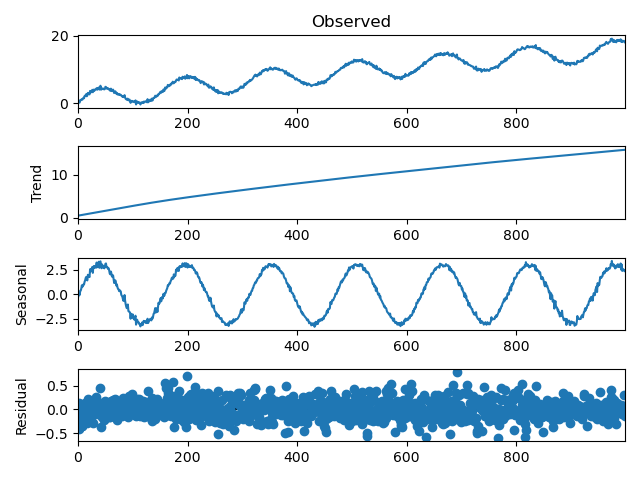
\includegraphics[width=0.7\textwidth]{imgs/stl1.png}
    \caption{$f(x) = x^{0.75} + 2\sin(x)$ with added noise
      $\sim \mathcal{N}(0, 0.25)$}
  \end{figure}
  \centering
\end{frame}


\begin{frame}
\frametitle{Locally Estimated Scatterplot Smoothing (LOESS)}
\begin{itemize}
  \item For all $x$ fit a curve $\hat{g}(x)$ by giving the other points $x_i$ a
  weight $v_i$.
\item Select the value of the smoothing factor $q \in \mathbb{Z}^+$ and let
  $\lambda_q(x)$ be the distance from $x$ to q'th farthest $x_i$.
\item We calculate the weights using the tricube weight function:
  \[
  v_i = \left( 1 - \left( \frac{| x_i - x |}{\lambda_q(x)}  \right)^3\right)^3
  \]
  for $| x_i - x | \geq \lambda_q(x)$, set $v_i = 0$
\item Use locally-linear or locally quadratic fitting with weights
  $\rho_i v_i$, where $\rho_i$ are the robustness weights that make it possible to 
  ignore the outliers in the dataset.
\item The value of $x$ after the application of LOESS is $\hat{g}(x)$,
\end{itemize}
\end{frame}

\begin{frame}
  \frametitle{LOESS Examples}
  \begin{figure}
    \centering
    \begin{subfigure}[b]{0.49\textwidth}
      \centering
      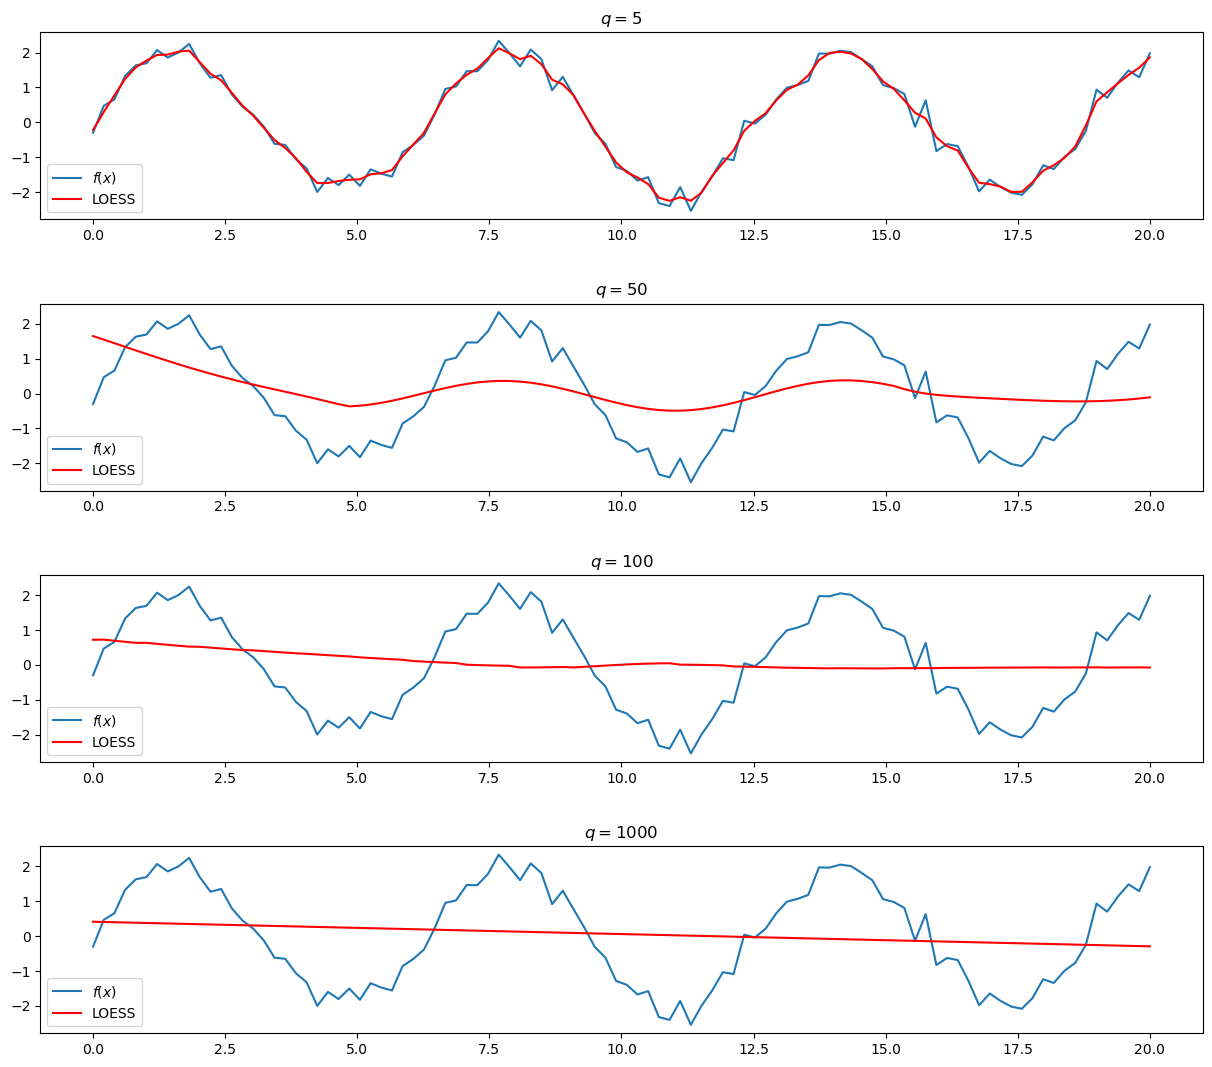
\includegraphics[width=\textwidth]{imgs/loess1}
      \caption{$d=1$}
  \end{subfigure}
  \begin{subfigure}[b]{0.49\textwidth}
    \centering
    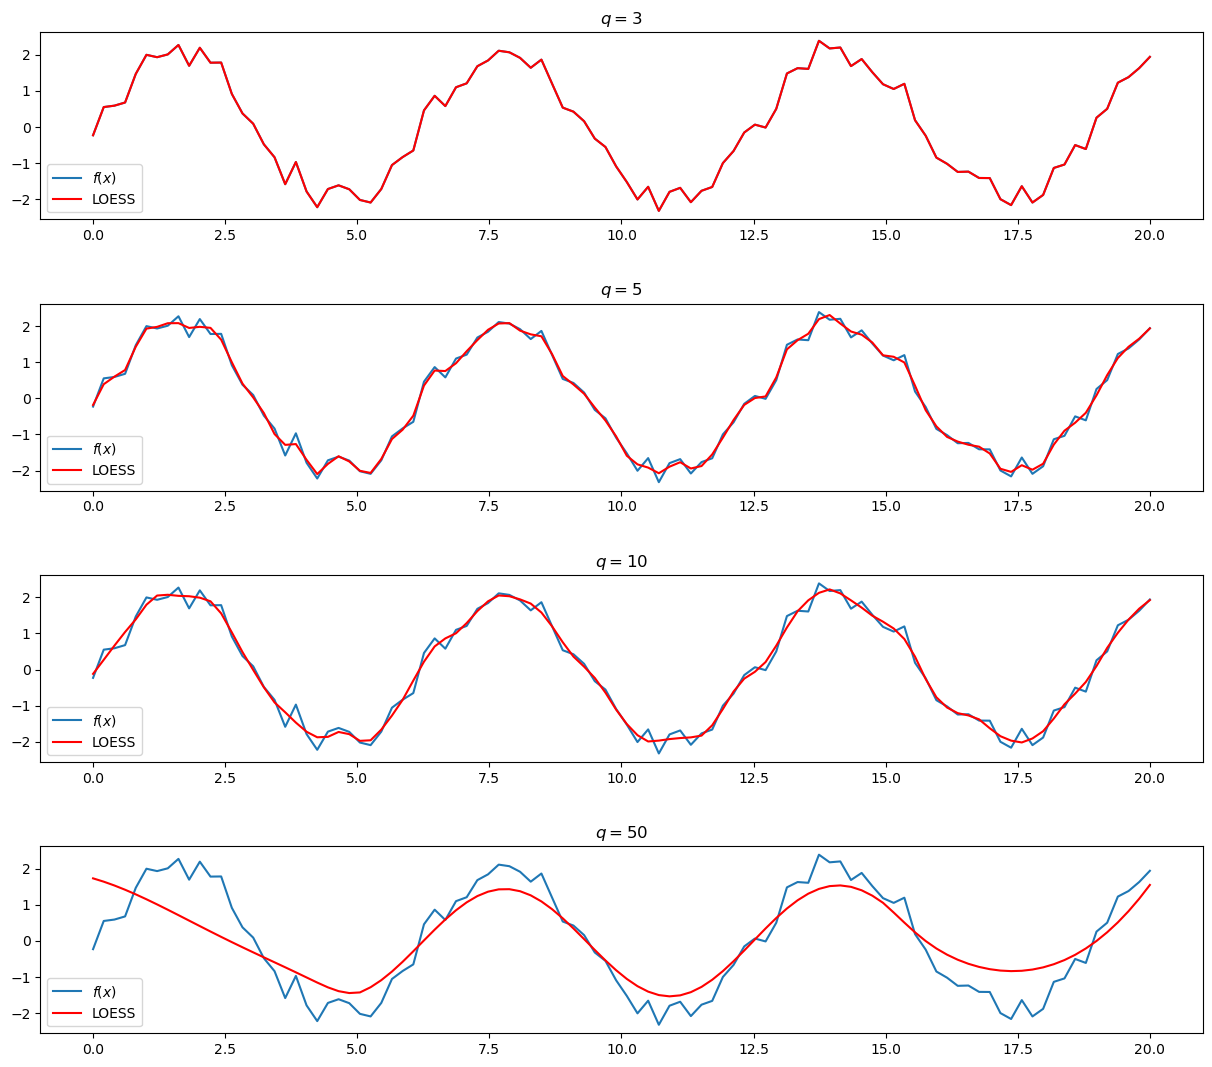
\includegraphics[width=\textwidth]{imgs/loess2}
    \caption{$d=2$}
  \end{subfigure}
  \caption{LOESS applied to $f(x) = 2\sin(x)$ with added Gaussian noise and $n =
    100$. $d$ is the degree of the fitted polynomial}
\end{figure}

\end{frame}

\begin{frame}
  \frametitle{STL Algorithm Steps}
  \begin{itemize}
  \item STL is performed through two nested loops and we begin by setting:
    \[ T_v^{0} = 0, \quad R_v^{0} = 0,  \quad \rho_v = 1 \]
  \item Inner Loop:
\begin{enumerate}
\item \textbf{Detrending}:
  $Y_v - T_v^k$, where $k$ is the iteration number.
\item \textbf{Cycle-Subseries Smoothing}:
  $Y_v - T_v^k$ is split into cycle-subseries.
  Take the mean of the seasonal component, resulting in 
  $C^{k+1}$.
\item \textbf{Low-pass Filter of Smoothed Cycle-Subseries}:
  Apply the low-pass filter to $C_{k+1}$. This is accomplished by application of two
  moving averages of lag equal to 3 followed by LOESS smoothing with $q=n_l$
  and $d=1$. The result is saved as $L^{k+1}$
\item \textbf{Detrending of the Smoothed Cycle-Subseries}:
  $S^{k+1} = C^{k+1} - L^{k+1}$
\item \textbf{Deseasoning}:
  $Y_v - S_v^k$. If a value of $Y_v$ is missing, the detrending value must also be missing.
\item \textbf{Trend Smoothing}:
  Apply LOESS to $Y_v - S_v^k$ with $q = n_t$, resulting in $T^{k+1}$
\end{enumerate}
  \end{itemize}
\end{frame}

\begin{frame}
  \frametitle{STL Algorithm Steps - Continued}
  \begin{itemize}
\item  The outer loop consists of following steps:
  \begin{enumerate}
  \item Run the inner loop
  \item Find the remainder:
    $R_v = Y_v - T_v - S_v$
  \item Calculate the robustness weights from the remainder component:
    \[
    \rho_{v}= B\left( \frac{|R_v|}{6\cdot\text{median}(|R_v|)} \right)
    \]
    where $B$ is the bisquare weight function:
    \[
    B(x) =
    \begin{cases}
      \left(1-x^{2}\right)^{2} & \text{ for } 0 \leqslant x<1 \\
      0                     & \text{ for } x>1
    \end{cases}
    \]
\end{enumerate}
  \end{itemize}
\end{frame}


\begin{frame}
\frametitle{OLS-MOSUM Test}
\begin{itemize}
  \item Model
\end{itemize}
\end{frame}

\begin{frame}
\frametitle{Breakpoint Detection Algorithm}
\begin{itemize}
  \item Described in the paper by Bai and Perron from 2003
\end{itemize}
\end{frame}

\begin{frame}
\frametitle{BFAST}
\begin{block}{Block Title}
Lorem ipsum dolor sit amet, consectetur adipisicing elit, 
sed do eiusmod tempor incididunt ut labore et 
dolore magna aliqua.
\end{block}
\begin{itemize}
  \item Model
\end{itemize}
\end{frame}

\begin{frame}
\frametitle{\texttt{nile} dataset}
\begin{figure}[H]
  \centering
  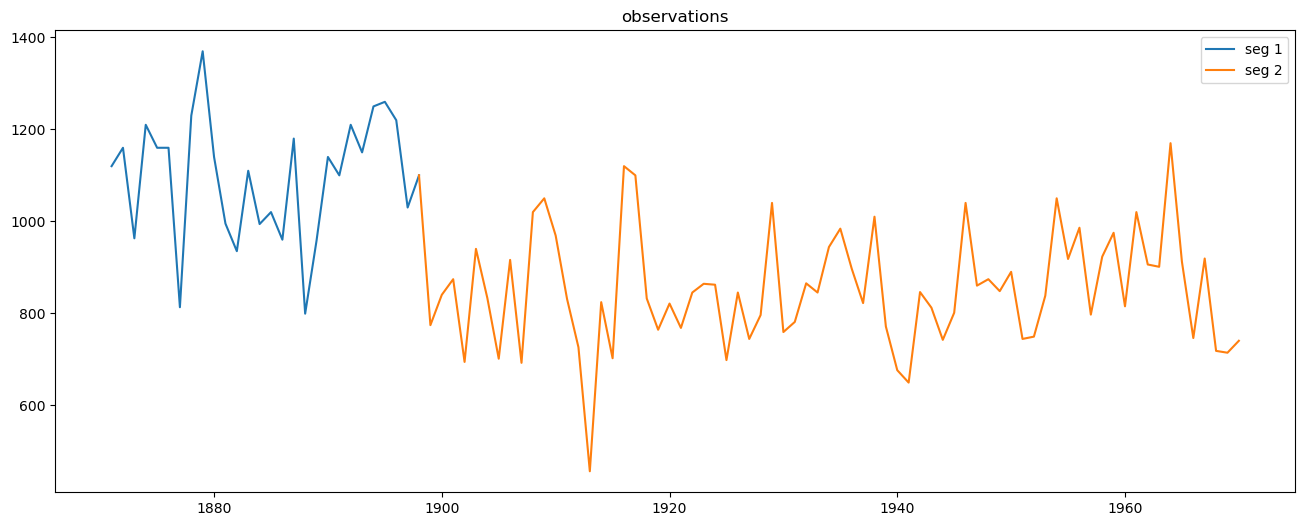
\includegraphics[width=0.9\textwidth]{imgs/nile.png}
\end{figure}
\end{frame}

\begin{frame}
\frametitle{\texttt{harvest} dataset}
\begin{figure}[H]
  \centering
  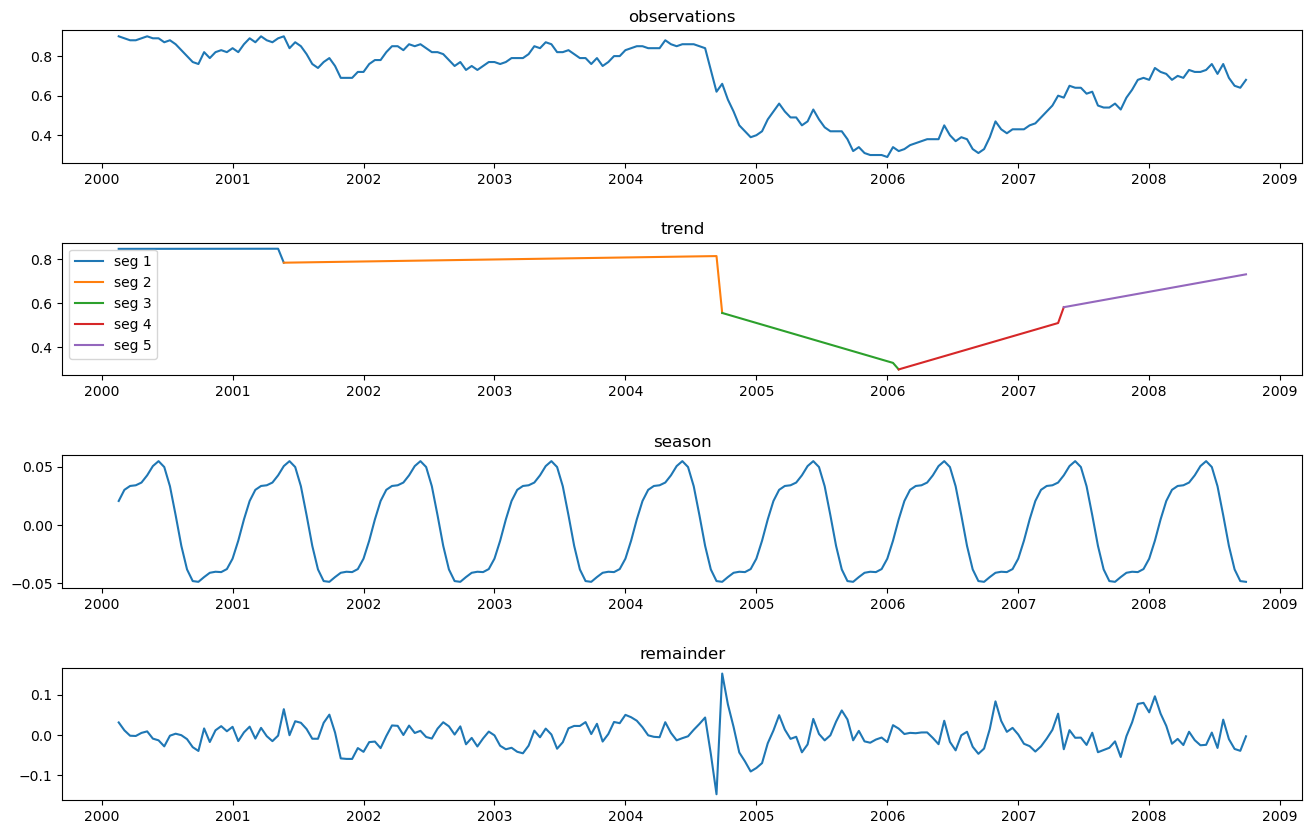
\includegraphics[width=0.9\textwidth]{imgs/harvest.png}
\end{figure}
\end{frame}


\begin{frame}
\frametitle{\texttt{simts} dataset}
\begin{figure}[H]
  \centering
  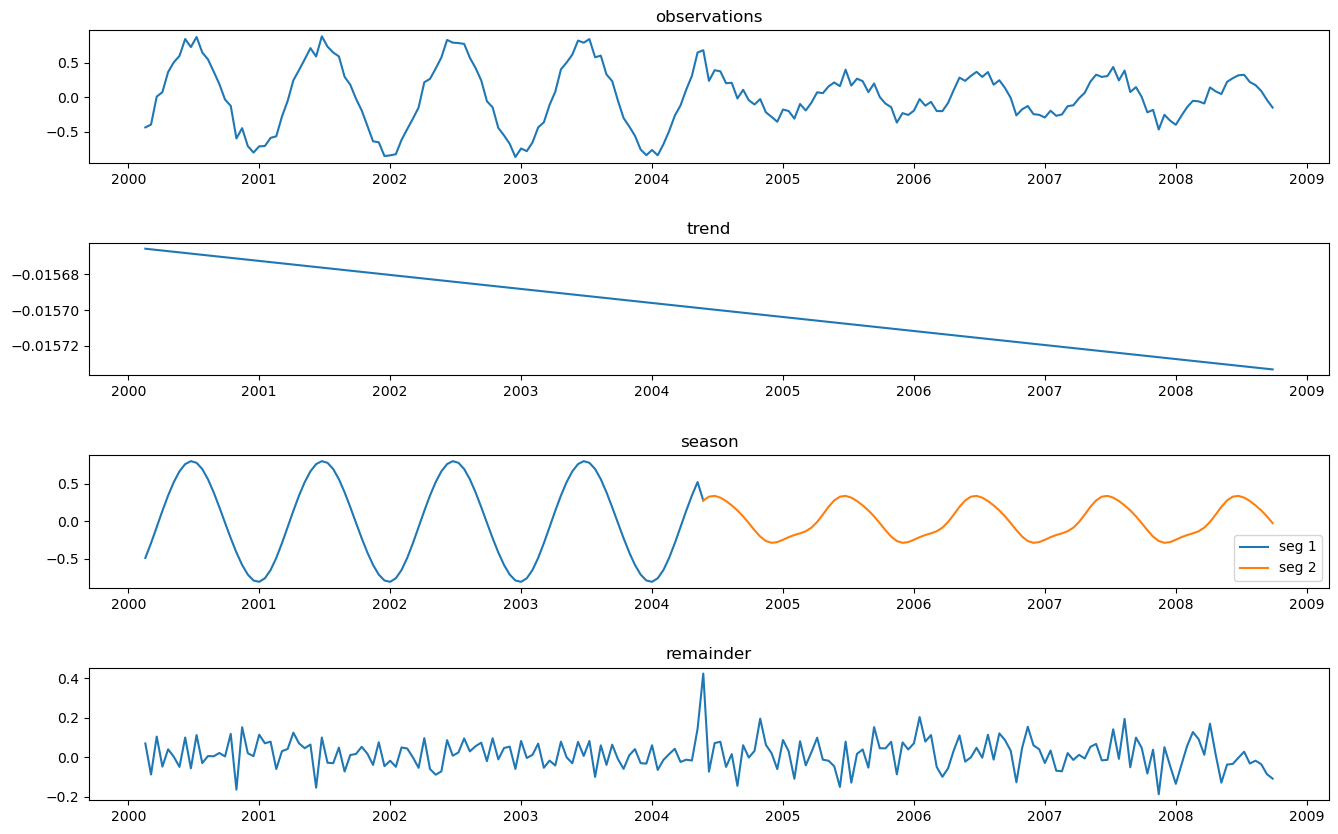
\includegraphics[width=0.9\textwidth]{imgs/simts.png}
\end{figure}
\end{frame}

\begin{frame}
\frametitle{\texttt{ndvi} dataset}
\begin{figure}[H]
  \centering
  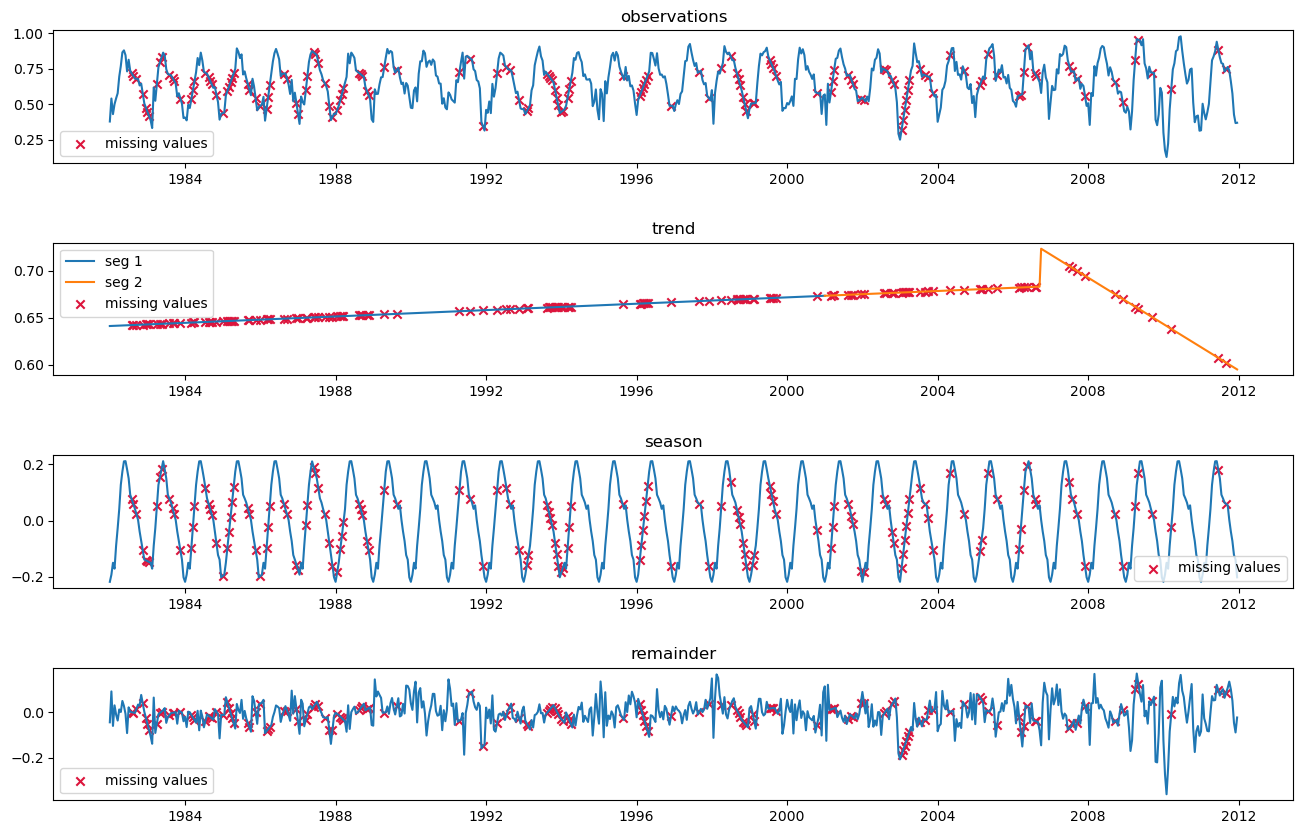
\includegraphics[width=0.9\textwidth]{imgs/ndvi.png}
\end{figure}
\end{frame}

\begin{frame}
\frametitle{Links}
\centering
\begin{itemize}
\item Full project report can be found here:\\
  \url{https://raw.githubusercontent.com/mortvest/bfast-py/master/report/main.pdf}
\item The source code can be found in the GitHub repository:\\
  \url{http://github.com/mortvest/bfast-py}
\end{itemize}
\end{frame}

\begin{frame}
  \frametitle{Questions}
  \centering 
  \Huge ?
\end{frame}

%% \begin{frame}
%%   \frametitle{All results RTX 2080Ti (EXTRA)}
%% \begin{figure}[H]
%%   \centering
%%   \begin{subfigure}[t]{0.4\textwidth}
%%     \centering
%%     \includegraphics[width=\textwidth]{imgs/RTX_2080_Ti_scansubblock.eps}
%%   \end{subfigure}
%%   \begin{subfigure}[t]{0.4\textwidth}
%%     \centering
%%     \includegraphics[width=\textwidth]{imgs/RTX_2080_Ti_flagAggrVal.eps}
%%   \end{subfigure}
%%   \begin{subfigure}[t]{0.4\textwidth}
%%     \centering
%%     \includegraphics[width=\textwidth]{imgs/RTX_2080_Ti_scansubblockexcl.eps}
%%   \end{subfigure}
%% \end{figure}
%% \end{frame}

\end{document}



